\begin{figure}[htbp]
\centering
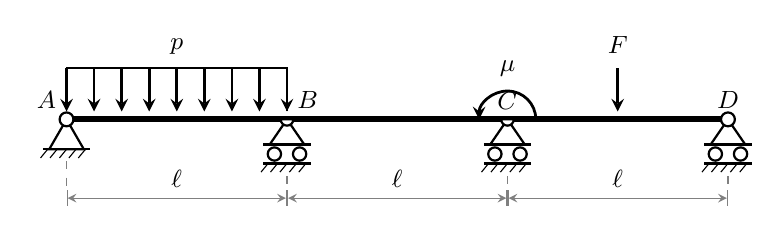
\begin{tikzpicture}[>=stealth, line width=0.8pt, font=\small,
	nodo/.style={circle, fill=white, draw=black,
		inner sep=0pt, minimum size=5pt, line width=0.8pt},
	carr/.style={->, >=stealth, line width=1.0pt, black},
	quota/.style={thin, gray, |<->|},
	richiam/.style={thin, gray, dashed},
	]
	
	\def\L{2.80}    % lunghezza campata
	\def\tw{0.22}   % semi-larghezza triangolo
	\def\thA{0.38}  % altezza triangolo cerniera A
	\def\thR{0.32}  % altezza triangolo carrello
	\def\rn{0.08}   % raggio semicerchio appoggi intermedi B, C
	\def\bw{0.16}   % semi-distanza ruote carrello
	\def\gw{0.30}   % semi-larghezza barra di terra
	\def\yd{-1.00}  % quota linee di misura
	
	%% ── Trave ────────────────────────────────────────────────────────────────
	\draw[line width=2.2pt](0,0)--({3*\L},0);
	
	%% ── Fibre inferiori ──────────────────────────────────────────────────────
	%\draw[line width=0.6pt, dashed, gray!55](0,-0.15)--({3*\L},-0.15);
	
	%% ── Etichette nodi ───────────────────────────────────────────────────────
	\node[above left =0.04]at(0,0){$A$};
	\node[above right=0.04]at({\L},0){$B$};
	\node[above=-0.08]at({2*\L},0){$C$};
	\node[above=0.04]at({3*\L},0){$D$};
	
	%% ── Cerniera A ───────────────────────────────────────────────────────────
	\draw(0,0)--++(-\tw,-\thA)--++(2*\tw,0)--cycle;
	\draw({-\gw},{-\thA})--(\gw,{-\thA});
	\foreach \x in {-0.24,-0.12,0,0.12,0.24}
	\draw[thin](\x,{-\thA})--++(-.09,-.11);
	\node[nodo]at(0,0){};
	
	%% ── Appoggio intermedio B (semicerchio = continuità rotazionale) ──────────
	\draw({\L},0)--++(-\tw,-\thR)--++(2*\tw,0)--cycle;
	\draw({\L-\gw},{-\thR})--({\L+\gw},{-\thR});
	\draw({\L-\bw},{-\thR-0.12})circle(2.4pt);
	\draw({\L+\bw},{-\thR-0.12})circle(2.4pt);
	\draw({\L-\gw},{-\thR-0.24})--({\L+\gw},{-\thR-0.24});
	\foreach \x in {-0.24,-0.12,0,0.12,0.24}
	\draw[thin]({\L+\x},{-\thR-0.24})--++(-.09,-.11);
	\draw[fill=white]({\L-\rn},0) arc(180:360:\rn)--cycle;
	
	%% ── Appoggio intermedio C (semicerchio = continuità rotazionale) ──────────
	\draw({2*\L},0)--++(-\tw,-\thR)--++(2*\tw,0)--cycle;
	\draw({2*\L-\gw},{-\thR})--({2*\L+\gw},{-\thR});
	\draw({2*\L-\bw},{-\thR-0.12})circle(2.4pt);
	\draw({2*\L+\bw},{-\thR-0.12})circle(2.4pt);
	\draw({2*\L-\gw},{-\thR-0.24})--({2*\L+\gw},{-\thR-0.24});
	\foreach \x in {-0.24,-0.12,0,0.12,0.24}
	\draw[thin]({2*\L+\x},{-\thR-0.24})--++(-.09,-.11);
	\draw[fill=white]({2*\L-\rn},0) arc(180:360:\rn)--cycle;
	
	%% ── Carrello D ───────────────────────────────────────────────────────────
	\draw({3*\L},0)--++(-\tw,-\thR)--++(2*\tw,0)--cycle;
	\draw({3*\L-\gw},{-\thR})--({3*\L+\gw},{-\thR});
	\draw({3*\L-\bw},{-\thR-0.12})circle(2.4pt);
	\draw({3*\L+\bw},{-\thR-0.12})circle(2.4pt);
	\draw({3*\L-\gw},{-\thR-0.24})--({3*\L+\gw},{-\thR-0.24});
	\foreach \x in {-0.24,-0.12,0,0.12,0.24}
	\draw[thin]({3*\L+\x},{-\thR-0.24})--++(-.09,-.11);
	\node[nodo]at({3*\L},0){};
	
	%% ── Carico distribuito p su AB ───────────────────────────────────────────
	\draw[line width=0.5pt](0,0.10)--(0,0.65)--({\L},0.65)--({\L},0.10);
	\foreach \k in {0,1,2,3,4,5,6,7,8}{
		\pgfmathsetmacro{\xk}{\k*(\L/8.0)}
		\draw[carr]({\xk},0.65)--({\xk},0.10);}
	\node[font=\small,above]at({0.5*\L},0.70){$p$};
	
	%% ── Coppia μ in C: semicerchio sopra, convessità verso l'alto ────────────
	\def\rmu{0.36}
	\draw[->,>=stealth,line width=1.0pt]({2*\L+\rmu},0) arc(0:180:\rmu);
	\node[font=\small,above]at({2*\L},{\rmu+0.05}){$\mu$};
	
	%% ── Forza F a mezzeria CD ────────────────────────────────────────────────
	\draw[carr]({2.5*\L},0.65)--({2.5*\L},0.10);
	\node[font=\small,above]at({2.5*\L},0.70){$F$};
	
	%% ── Quotatura ────────────────────────────────────────────────────────────
	\draw[richiam](0,{-\thA-0.15})--(0,{\yd+0.08});
	\draw[richiam]({\L},{-\thR-0.40})--({\L},{\yd+0.08});
	\draw[richiam]({2*\L},{-\thR-0.40})--({2*\L},{\yd+0.08});
	\draw[richiam]({3*\L},{-\thR-0.40})--({3*\L},{\yd+0.08});
	\draw[quota](0,{\yd})--({\L},{\yd});
	\node[font=\small,above=0.04]at({0.5*\L},{\yd}){$\ell$};
	\draw[quota]({\L},{\yd})--({2*\L},{\yd});
	\node[font=\small,above=0.04]at({1.5*\L},{\yd}){$\ell$};
	\draw[quota]({2*\L},{\yd})--({3*\L},{\yd});
	\node[font=\small,above=0.04]at({2.5*\L},{\yd}){$\ell$};
	
\end{tikzpicture}
\caption{Trave continua a tre campate di uguale luce $\ell$:
	carico uniformemente distribuito $p$ sul tratto $AB$,
	coppia concentrata $\mu$ nella sezione $C$,
	forza concentrata $F$ a mezzeria del tratto $CD$.
	Il cerchio in $A$ e $D$ indica il perno; il semicerchio in $B$ e $C$
	indica che la trave scorre sull'appoggio senza interruzione
	della continuità rotazionale.}
\label{fig:tc_schema}
\end{figure}
